\documentclass{beamer}
%
\usepackage{beamerthemesplit}
\usepackage{cite}
\usepackage{graphicx}
\usepackage{times}
\usepackage{amsmath,amsfonts,amssymb}
\usepackage{psfrag,latexsym,stmaryrd,color,bbm,mathrsfs}
%
\mode<presentation> { \usetheme{Warsaw} }
%
\title{Computational models for\\ quantum computation}
\author{Pascal Steger}
\date[10. 03. 2008]{Proseminar in theoretical physics, 2008}
%
%\pgfdeclaremask{eth}{ethlogo_kurz}
\pgfdeclareimage[width=1cm]{ethlogo_kurz}{ethlogo_kurz}
%
\logo{\pgfuseimage{ethlogo_kurz}}
% 
\begin{document}
%
\begin{frame}
    \titlepage
\end{frame}
%
%
\section{Introduction}
%
\subsection{overview}
\begin{frame}
    \tableofcontents
\end{frame}
%
\subsection{literature}
\begin{frame}
    \bibliographystyle{plain}
    \bibliography{qc_bib}
    % in order to display all literature: reference articles, books
	% shows up as [1] [2] [3] [4]
	\hfill\vfill
	\cite{benioff1998}
	\cite{deutsch1985}
	\cite{deutsch1989}
%   \cite{kaye2007}
	\cite{yao1993}
\end{frame}
%
\subsection{two basic models}
\begin{frame}
	\frametitle{two models}
    \begin{block}{two basic models for quantum computation}<1->
	    \begin{itemize}
    	    \item<2-> quantum computational network, built of quantum gates
        	\item<2-> Quantum Turing Machine
    	\end{itemize}
	\end{block}
	\begin{block}{connections between models}<3->
		\begin{itemize}
			\item<4-> quantum mechanical description: step operator
			\item<4-> complexity theory
		\end{itemize}
	\end{block}
\end{frame}
%
\begin{frame}
	\tableofcontents
\end{frame}
%
%
\section{Quantum Gates}
%
\subsection[logic circuits]{}
\begin{frame}
	\frametitle{general definitions}
	\begin{description}
		\item[computation:] process that produces output depending on input
		\item[in-,output:] abstract symbols
		\item[bit,quantum:] smallest possible quantity of non-probabilistic information
		\item[carrier:] physical representation of a bit, e.g. spin $1/2$-particle
	\end{description}
\end{frame}
%
\begin{frame}
	\frametitle{logic circuits}
	\begin{figure}
		\centering
		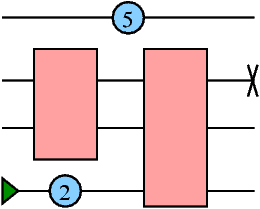
\includegraphics[width=2.5cm]{logic_circuit.png}
	\end{figure}
	\begin{description}
		\item[logic circuit:]<1-> computing machine consisting of logic gates; computational steps synchronized; outputs$(i)$=inputs$(i+1)$; can use sources and sinks
		\item[source:]<2-> gate with only one output that emits $0$ or $1$ in each step; reversible
		\item[sink:]<2-> gate with only one input that deletes information; irreversible
		\item[unit wire:]<2-> computes identity function with fixed time dilation
	\end{description}
\end{frame}
%
\begin{frame}
	\begin{block}{physical processes in quantum computer}
		\begin{enumerate}
			\item preparation of input states in carriers
			\item as a black box:
			\item QM elastic scattering (errorless)
			\item measurement of output carriers after fixed step
		\end{enumerate}
	\end{block}
\end{frame}
%
\subsection{definitions}
\begin{frame}
	\frametitle{gates: definitions}
    \begin{description}
        \item[logic gate:]<1-> computing machine; input and output consist of fixed number of bits; fixed computation is done in fixed time.
        \item[quantum gate:]<1-> states of input and output can be quantum mixtures of eigenstates of input observable $\hat{I}$ and output observable $\hat{O}$.
		\item[reversible gate:]<2-> inputs and outputs are related by invertible function (ideal case, no errors)
	\end{description}
\end{frame}
%
%\subsection{mathematical description}
\begin{frame}
	\frametitle{mathematical descriptions of gates}
	\begin{block}{computational basis:}
		eigenstates of $\hat{I}$ and $\hat{O}$ in Schr\"odinger picture, if they coincide.
	\end{block}
    \begin{itemize}
    \item by table
    \item by permutation: let $\{|a,b\rangle\},\quad a,b\in\{0,1\}$ be the four computational basis states. A gate transforms inputs into outputs, e.g.
        \begin{table}\label{XOR}
            \begin{tabular}{rcl}
                $|0,0\rangle$&$\to$&$|0,0\rangle$\\
                $|0,1\rangle$&$\to$&$|1,1\rangle$\\
                $|1,0\rangle$&$\to$&$|1,0\rangle$\\
                $|1,1\rangle$&$\to$&$|0,1\rangle$
            \end{tabular}
        \end{table}
    \item by $S$-Matrix, more suitable for quantum gates
    \end{itemize}
\end{frame}
%
%\subsection{examples}
\begin{frame}
    \frametitle{example: C-NOT, measurement gate}
    \begin{figure}
		\centering
        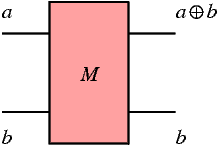
\includegraphics[width=3cm]{mGate.png}
%        \caption{measurement gate - its own reverse}
    \end{figure}
    \begin{table}
        \begin{tabular}{rr|cc|cl}
            $a$&$b$&$a\oplus b$&$b$&$(a\oplus b)\oplus b$&$b$\\
            \hline\hline
            0&0&0&0&0&0\\
            0&1&1&1&0&1\\
            1&0&1&0&1&0\\
            1&1&0&1&1&1
        \end{tabular}
    \end{table}
\end{frame}
%
\begin{frame}
	\frametitle{$S$-matrix}
	\begin{itemize}
		\item $S_{a'b'\ldots}^{ab\ldots}$ has clumped indices $ab\ldots$, $a'b'\ldots$ denoting the states of the input and output carriers
		\item operation of gate corresponds to matrix multiplication with $S_{a'b'\ldots}^{ab\ldots}$
		\begin{equation}
            |a,b,\ldots\rangle\to\sum_{a',b',\ldots\in\{0,1\}} S_{a'b'\ldots}^{ab\ldots}|a',b',\ldots\rangle\equiv S|a,b,\ldots\rangle.
		\end{equation}
		\item repeated gates are represented by powers of $S$
		\item $S$ can also denote linear operator if no basis chosen
	\end{itemize}
\end{frame}
%
\begin{frame}
	\frametitle{example: NOT-gate}
	\begin{figure}
		\centering
		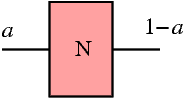
\includegraphics[width=2cm]{not.png}
%    \caption{NOT gate}
	\end{figure}
	\begin{eqnarray}
		S_N&=&\begin{pmatrix}0&1\\1&0\end{pmatrix}\\
		S_{N^\alpha}&=&S_N^\alpha=\frac{1}{2}\begin{pmatrix}1+e^{i\pi\alpha}&1-e^{i\pi\alpha}\\1-e^{i\pi\alpha}&1+e^{i\pi\alpha}\end{pmatrix}
	\end{eqnarray}
%explain: NOT \alpha times is \alpha times S
	\begin{itemize}
		\item $\alpha\notin\mathbb{N}$: $N^\alpha$ is a power of NOT
		\item $\alpha\in\mathbb{N}$: $N^\alpha$ is a logic gate: identity or NOT
	\end{itemize}
\end{frame}
%
\subsection{Toffoli- and $Q$-gate}
\begin{frame}
	\frametitle{Toffoli gate in quantum computation}
	\begin{figure}
		\centering
		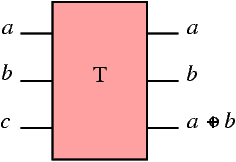
\includegraphics[width=2.5cm]{toffoli.png}
	\end{figure}
	\begin{itemize}
		\item<1-> classical gate: Toffoli
		\begin{equation}
			S_{Ta'b'c'}^{abc}=\delta_{a'}^a\delta_{b'}^b[(1-ab)\delta_{c'}^c+ab(S_N)_{c'}^c]
		\end{equation}
		\item<2-> analogon: quantum gate $Q$
		\begin{equation}
			S_{Qa'b'c'}^{abc}=\delta_{a'}^a\delta_{b'}^b\left[(1-ab)\delta_{c'}^c+iab e^{-i\pi\alpha/2}(S_N^\alpha)_{c'}^c\right]
		\end{equation}
	\end{itemize}
\end{frame}
\begin{frame}
	\frametitle{$S$-matrix of Toffoli and $Q$-gate}
	basis $0=|000\rangle$, $1=|001\rangle$, $\ldots$, $6=|110\rangle$, $7=|111\rangle$
	\begin{eqnarray*}
		S_T&=&\begin{pmatrix}
				\mathbbm{1}&&\\
				&0&1\\
				&1&0
		      \end{pmatrix}\\
		S_Q&=&\begin{pmatrix}
		       \mathbbm{1}&&\\
				&i\cos\pi\alpha/2&\sin\pi\alpha/2\\
				&\sin\pi\alpha/2&i\cos\pi\alpha/2
		      \end{pmatrix}
	\end{eqnarray*}
\end{frame}
%
\subsection{universality}
%\subsection{example: NOT}
\begin{frame}
    \frametitle{example NOT}
    \begin{eqnarray}
        S_{N^2}&=&S_N^2=\mathbbm{1},\\
        (S_{N^\alpha})^m&=&S_N^{m\alpha}=S_N^{m\alpha-2\lfloor m\alpha/2\rfloor}.
	\end{eqnarray}
	exponent $1+\varepsilon$ arbitrarily close to $1$, but never exact for $\alpha$ irrational, $m\in\mathbb{N}$.
	\begin{block}{time before non-classical behaviour:}
		\begin{equation*}
			t=\frac{1}{\max_{|\Psi\rangle}(1-|\langle\Psi|S_N^\dagger S_{N^\alpha}^m|\Psi\rangle|^2)}= \frac{1}{\sin^2\pi\varepsilon/2}\sim\varepsilon^{-2}\stackrel{(\varepsilon\to0)}\to\infty
    	\end{equation*}
	\end{block}
\end{frame}
\begin{frame}
    \frametitle{universality: definitions}
    \begin{description}
    	\item[computationally equivalent:]<1-> same output for same input
		\item[problem:]<1-> exact equivalence in QM not possible, e.g. NOT
        \item[adequate sets:]<2-> $F$ and $G$, if $\forall f\in F\,\exists \{g_n\in
        G\}$ and sequence $\{\phi_n\}$ of phase angles such that
        \begin{equation}
			\lim_{n\to\infty} S_{g_n} e^{i\phi_n}=S_f
		\end{equation}
		\item[example:]<2-> $F=\{N\}$ and $G=\{N^\alpha,\mathbbm{1}\}$ are adequate
        \item[universal gate:]<3-> quantum gate such that set of unit wire, source and this gate is adequate to set of other gates
    \end{description}
\end{frame}
%
%\subsection{universal q-gate}
\begin{frame}
    \begin{block}{Claim:}<1->
		The $Q$-gate is universal to set of all quantum gates.
	\end{block}
    \begin{block}{Proof:}<2->
     	create repetoire of gates that $Q$ is adequate to:
	    	\begin{enumerate}
    	    	\item Toffoli gate
        		\item all logic gates
        		\item all $3$-bit quantum gates
        		\item all $n$-bit quantum gates
        		\item all quantum gates
    		\end{enumerate}
    \end{block}
\end{frame}
\begin{frame}
	\frametitle{proof: step 1,2: Toffoli gate}
    choose basis
    $0=|000\rangle$, $1=|001\rangle$, $\ldots$, $6=|110\rangle$, $7=|111\rangle$
    \begin{equation*}
        S_Q^{4n+1}=\begin{pmatrix}
			\mathbbm{1}&&\\
            &i\cos\pi\alpha (2n+1/2)&\sin\pi\alpha (2n+1/2)\\
            &\sin\pi\alpha(2n+1/2)&i\cos\pi\alpha(2n+1/2)
        \end{pmatrix}
    \end{equation*}
    $S_Q^{4n+1}=S_T$ for arguments $\pi(2m+1/2)$, $m\in\mathbb{N}$;\\
    arbitrarily close to Toffoli with $\pi\alpha(2n+1/2)$ for some $n\in\mathbb{N}$.\\
    Toffoli gate in repetoire, proof similar to that for NOT\\
    Toffoli universal for all logic gates $\Rightarrow$ all logic gates in repetoire
\end{frame}
\begin{frame}
	\frametitle{proof: step 3: 3-bit quantum gates}
    \begin{eqnarray*}
        S_Q^{4n}&=&\begin{pmatrix}\mathbbm{1}&&\\
            &\cos 2n\pi\alpha&-i\sin2n\pi\alpha\\
            &-i\sin2n\pi\alpha&\cos2n\pi\alpha
        \end{pmatrix}\\
        &\equiv&\begin{pmatrix}\mathbbm{1}&&\\
            &\cos \lambda&i\sin\lambda\\
            &i\sin\lambda&\cos\lambda
        \end{pmatrix}\equiv U_\lambda
    \end{eqnarray*}
    is in repetoire, since $\exists m\in\mathbb{N}:\,|2\pi n\alpha-2\pi m|<\varepsilon$ for $\varepsilon$ arbitrarily small
\end{frame}
\begin{frame}
    permutations: logic gates, in repetoire;\\
    limit of combinations of permutations and $U$ does also:
    \begin{eqnarray*}
        \lim_{n\to\infty}&&[P_{56}(U_{\sqrt{\lambda/n}}P_{57})^2(U_{-\sqrt{\lambda/n}}P_{57})^2P_{56}]^n\\
        &&=\begin{pmatrix}\mathbbm{1}&&\\&\cos\lambda&\sin\lambda\\&-\sin\lambda&\cos\lambda\end{pmatrix}\equiv V_\lambda\\
        \lim_{n\to\infty}&&[U_{\sqrt{\lambda/2n}}V_{\sqrt{\lambda/2n}}U_{-\sqrt{\lambda/2n}}V_{-\sqrt{\lambda/2n}}\\
        &&=\textrm{diag}(1,\ldots,1,e^{-i\lambda},e^{i\lambda})\equiv
        W_\lambda
    \end{eqnarray*}
    change in global phase factor does not change observable:
    %QQ true? what is not affected is the Erwartungswert
    \begin{equation*}
        X_\lambda\equiv\textrm{diag}(1,\ldots,1,e^{i\lambda})
    \end{equation*}
    $V_\lambda,W_\lambda,X_\lambda$ are in repetoire
\end{frame}
\begin{frame}
    \begin{eqnarray*}
     \nonumber |\Psi\rangle&=&\sum_{n=0}^7c_n|n\rangle,\quad\sum_{n=0}^7|c_n|^2=1\\
     Z_6[|\Psi\rangle]&:=&X_{-\arg(c_6c_7)/2}V_{-\arctan|c_6/c_7|}W_{-\arg(c_7/c_6)/2}\\
     |\Psi\rangle&\Rightarrow&\sum_{n=0}^5c_n|n\rangle+0+\sqrt{|c_6|^2+|c_7|^2}|7\rangle
    \end{eqnarray*}
	by analogy: $G:\,c_i\to0,i<7$, gate in repetoire. in general:
	\begin{eqnarray*}
	 S&=&\sum_{n=0}^7e^{i\sigma_n}|\Psi_n\rangle\langle\Psi_n|;\\
	 S&=&\prod_{n=0}^7S_{G^{-1}[|\Psi_n\rangle]}X_{\sigma_n}S_{G[|\Psi_n\rangle]}
	\end{eqnarray*}
	$Q$ is universal to all $3\times3$-matrices
\end{frame}
\begin{frame}
	\frametitle{proof: 4,5: $n$ bit gates}
	\begin{figure}
		\centering
		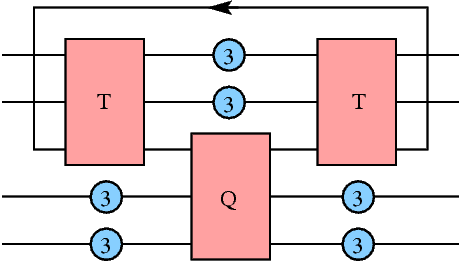
\includegraphics[width=4cm]{four_bit.png}
	\end{figure}
	\begin{itemize}
		\item loopback necessary to connect all inputs, outputs
		\item is initialized to $0$, output is $0$ again for all inputs
		\item makes circuit reversible, source and sink would yield irreversible gate
	\end{itemize}
	\begin{equation*}
     S_{Q_4a'b'c'd'}^{abcd}=\delta_{a'}^{a}\delta_{b'}^b\delta_{c'}^c[(1-abc)\delta_{d'}^d+iabc e^{-i\pi\alpha/2}(S_N^\alpha)_{d'}^d]
    \end{equation*}
    same procedure to get $n$-bit gates.\\
\end{frame}
%
%\subsection[summary]{}
\begin{frame}
	\frametitle{summary 1}
    \begin{block}{Most important}
        \begin{itemize}
			\item quantum gates can have superpositions of states as input
			\item $Q$-gate is universal wrt the set of all quantum gates
			\item proof constructs repetoire of gates that $Q$ is adequate to
		\end{itemize}
    \end{block}
\end{frame}
%
%
\section{Quantum Turing Machine}
%
\begin{frame}
 \tableofcontents
\end{frame}
%\subsection[definitions]{}
\begin{frame}
	\frametitle{Quantum Turing Machine (QTM)}
	\begin{block}{definition}
	    \begin{itemize}
			\item consists of a finite processor and an infinite memory
			\item computation proceeds in steps of fixed duration $T$
			\item only processor and finite part of memory interact
			\item \emph{halts}, if two subsequent states identical or halt flag set
			\item halt flag: observable, spectrum $\{0,1\}$, independent of $\hat{I}$.
			\item universal, can simulate any other quantum computer
		\end{itemize}
	\end{block}
	\begin{figure}
		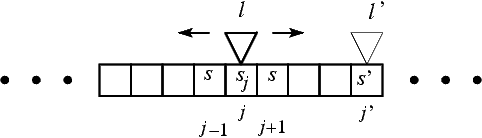
\includegraphics[width=4cm]{qtm.png}
	\end{figure}
\end{frame}
%
\subsection{Church-Turing}
\begin{frame}
    \begin{block}{Church-Turing hypothesis}
        Every function which would naturally be regarded as computable can be computed by the universal Turing machine.
    \end{block}
    \begin{block}{Church-Turing, physical principle}
        Every finitely realizible physical system can be perfectly simulated by a universal computing machine operating by finite means.
    \end{block}
    QTM fulfills this principle\\
	Turing machine does not fulfill second version, since it is finite, but systems are continuous
\end{frame}
%
\subsection{step operator}
\begin{frame}
    \begin{block}{step operator: single step of computation}
	    \begin{itemize}
    	    \item head interacts with tape only at one position in fixed time
        	\item head can move to the left, to the right, or stay and interact
	        \item description: unitary \emph{step} operator $T$
    	    \item requirements: locality, displacement in at most one direction,
    	    periodicity (lattice sites)
        	\begin{eqnarray*}
            	\langle l',j',s'|T|l,j,s\rangle&=&\langle s'_{\neq j}|s_{\neq j}\rangle\langle
            	l',j',s'_{j'}|\tilde{T}|l,j,s_j\rangle,\\
            	\tilde{T}&=&\sum_{j=-\infty}^\infty\sum_{\Delta=-1}^1
            	P_{j+\Delta}\tilde{T}P_j,\\
            	\langle
            	l',j'+\Delta,s'|\tilde{T}|l,j',s\rangle&=&\langle
            	l',j+\Delta,s'|\tilde{T}|l,j,s\rangle.
        	\end{eqnarray*}
    	\end{itemize}
    \end{block}
\end{frame}
%
\subsection{dynamics}
\begin{frame}
	\frametitle{Hamiltonian}
	\begin{enumerate}
	\item<1-> for gates (Deutsch):
		\begin{equation}
        	H\equiv\frac{i}{t}\ln S
    	\end{equation}
    \begin{itemize}
		\item $H$ is local; description complexity is relatively small
	\end{itemize}
	\item<2-> according Feynman:
    	\begin{equation}
        	H\equiv K(2-T-T^\dagger)
    	\end{equation}
	\begin{itemize}
		\item gives kinetic energy if $T$ is only displacement
		\item note: $T$ can be a sum of elementary, unitary step operators for single gates
    \end{itemize}
	\end{enumerate}
\end{frame}
%
%\subsection[summary]{}
\begin{frame}
	\frametitle{summary 2}
	\begin{block}{most important}
		\begin{itemize}
			\item QTM is quantum analogon to Turing machine
			\item fulfills the Church-Turing principle
			\item can be described by step operators and Hamiltonian
		\end{itemize}
	\end{block}
\end{frame}
\begin{frame}
 \tableofcontents
\end{frame}
%
%
\section{Complexity}
%
\subsection[definitions]{}
\begin{frame}
	\frametitle{complexity: definitions}
	\begin{description}
		\item[size:]<1-> number of elementary gates in a quantum circuit
		\item[depth:]<1-> max. length of a directed path from in- to output
		\item[interacting pair of quantum circuits:]<2-> partition of circuit with disjoint sets of inputs, all outputs on one side
		\item[communication cost:]<2-> no. wires between interacting pairs
		\item[$(n,t)$-simulation:]<3-> of a QTM $M$ by a quantum circuit $C$, if input $\tilde{x}\in\{0,1\}^n$ evolved by $C$ is the same as
		the state of $M$ after $t$ steps
	\end{description}
\end{frame}
%
\subsection{theorems}
\begin{frame}
	\frametitle{theorems by Yao}
	\begin{enumerate}
		\item unitary operator $U\in\mathbb{C}^{2^n}$ can be simulated by quantum network using $2^{\mathcal{O}(n)}$ 3-gates, with $\mathcal{O}(n)$ wires
		\item every QTM can be $(n,t)$-simulated by a quantum network of size $poly(n,t)$
		\item $\exists$ universal QTM that can simulate any other QTM with only polynomial slowdown
	\end{enumerate}
\end{frame}
%
\subsection{Everett's interpretation; stock market}
\begin{frame}
	\begin{block}{Everett's interpretation}<1->
		computation takes place in parallel universes
	\end{block}
	\begin{block}{application}<2->
		stock market:
		\begin{itemize}
			\item input: stocks of today
			\item calculate a time $t$ to predict new stocks
			\item failure with 50\%
			\item other 50\% yield result of calculation time $2t$
			\item in average computation times are the same
		\end{itemize}
	\end{block}
\end{frame}
%
%\subsection[summary]{}
\begin{frame}
	\frametitle{summary 3}
	\begin{block}{most important}
		\begin{itemize}
			\item<1-> QTM can be simulated by quantum circuit or other QTM with polynomial slowdown
			\item<2-> quantum computer "calculates in parallel universes", not faster in average
		\end{itemize}
	\end{block}
\end{frame}
%
\begin{frame}
	\tableofcontents
\end{frame}
%
\begin{frame}
	\frametitle{discussion}
	\begin{block}{questions...}
		answers...
	\end{block}
\end{frame}
%
\end{document}
